\paragraph{QuizziPedia::Back-End::App::Models::TopicModel}
\label{QuizziPedia::Back-End::App::Models::TopicModel}
\begin{figure}[ht]
	\centering
	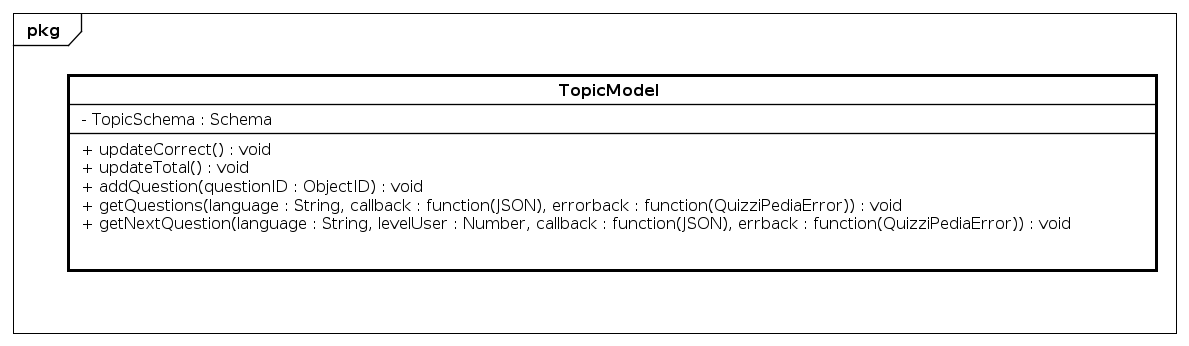
\includegraphics[scale=0.6]{UML/Classi/Back-End/QuizziPedia_Back-End_App_Models_topicModel.png}
	\caption{QuizziPedia::Back-End::App::Models::TopicModel}
\end{figure}
\FloatBarrier
\begin{itemize}
	\item \textbf{Descrizione}: classe che modella gli argomenti all'interno delle domande;
	\item \textbf{Utilizzo}:	viene utilizzata per rappresentare i dati relativi agli argomenti delle domande. Si interfaccia con la libreria \textit{Mongoose\ped{G}} per la creazione dello schema e dei relativi metodi statici o di istanza;
	\item \textbf{Relazioni con altre classi}:
		\begin{itemize}
			\item \textbf{IN \texttt{TopicController}} \\
			Classe che gestisce la logica applicativa riguardante la visualizzazione e la modifica degli argomenti delle domande;
			\item \textbf{OUT \texttt{QuestionModel}} \\
			Questa classe rappresenta i dati delle domande create dai vari utenti.
		\end{itemize}
	\item \textbf{Attributi}:
		\begin{itemize}
			\item \texttt{- topicSchema: Schema} \\
			Questo campo dati rappresenta lo schema \textit{Mongoose\ped{G}} per gli argomenti e prevede i seguenti attributi:
				\begin{itemize}
					\item \texttt{name: String}\\ Rappresenta il nome dell'argomento;
					\item \texttt{correctAnswers: Number}\\ Rappresenta il numero totale di domande alle quali gli utenti hanno risposto correttamente durante un allenamento sull'argomento; 
					\item \texttt{totalAnswers: Number}\\ Rappresenta il numero totale di domande alle quali gli utenti hanno risposto durante un allenamento sull'argomento;
					\item \texttt{question: Array}\\ Array che ontiene gli \texttt{ObjectId} delle domande sull'argomento.
				\end{itemize}
		\end{itemize}
	\item \textbf{Metodi}:
		\begin{itemize}
			\item \texttt{+ updateCorrect() : void} \\
			Metodo che consente di tenere aggiornato il numero di risposte esatte date a domande sull'argomento;
			\item \texttt{+ updateTotal() : void} \\
			Metodo che consente di tenere aggiornato il numero totale di risposte date a domande sull'argomento;
			\item \texttt{+ addQuestion(questionId : ObjectID) : void} \\
			Metodo che consente di aggiunge una domanda tra le domande sull'argomento. \\
			\textbf{Parametri}:
			\begin{itemize}
			\item \texttt{questionId : ObjectId} \\
			Rappresenta l'identificativo della domanda da aggiungere.
			\end{itemize}
			\item \texttt{+ getQuestions(language : String, keyword : [String], \\callback : function(JSON), errback : function(QuizziPediaError))} \\
			Metodo che consente di ottenere le domande sull'argomento attraverso la funzione di \textit{callback\ped{G}} oppure un messaggio di errore. \\
			\textbf{Parametri}:
			\begin{itemize}
			\item \texttt{language : String} \\
			Rappresenta la lingua in cui sono scritte le domande che si vuole ottenere;
			\item \texttt{keyword : Array<String>} \\
			Rappresenta le keyword che possono essere assegnate alle domande che si vuole ottenere;
			\item \texttt{callback : function(JSON)} \\
			Rappresenta la \textit{callback\ped{G}} che il metodo deve chiamare al termine dell'elaborazione nel caso in cui non si siano verificati errori;
			\item \texttt{errback : function(QuizziPediaError)} \\
			Rappresenta la \textit{callback\ped{G}} che il metodo deve chiamare qualora si verificassero errori durante l'esecuzione del metodo.
			\end{itemize}
			\item \texttt{+ getNextQuestion(language : String, levelUser : Number, \\callback : function(JSON), errback : function(QuizziPediaError)):: void} \\
			Metodo che consente di ottenere la domanda successiva nella modalità allenamento, in base al livello dell'utente che lo sta svolgendo. \\
			\textbf{Parametri}:
			\begin{itemize}
			\item \texttt{language : String} \\
			Rappresenta la lingua in cui è scritta la domanda che si vuole ottenere;
			\item \texttt{levelUser : Number} \\
			Rappresenta il livello dell'utente che sta svolgendo l'allenamento;
			\item \texttt{callback : function(JSON)} \\
			Rappresenta la \textit{callback\ped{G}} che il metodo deve chiamare al termine dell'elaborazione nel caso in cui non si siano verificati errori;
			\item \texttt{errback : function(QuizziPediaError)} \\
			Rappresenta la \textit{callback\ped{G}} che il metodo deve chiamare qualora si verificassero errori durante l'esecuzione del metodo.
			\end{itemize}
		\end{itemize}
\end{itemize}